\chapter{三次曲线与群运算律}

\section{参数化三次曲线的例子}

一些平面三次曲线可以像二次曲线一样被参数化：

有结点的三次曲线 \(C: y^2 = x^3 + x^2 \subset \mathbb{R}^2\) 是由映射 \(\varphi: \mathbb{R}^1 \to \mathbb{R}^2\) 给出的像，其表达式为 \(t \mapsto (t^2 - 1, t^3 - t)\)（请自行验证）；

尖点三次曲线 \(C: y^2 = x^3 \subset \mathbb{R}^2\) 是由映射 \(\varphi: \mathbb{R}^1 \to \mathbb{R}^2\) 给出的像，其表达式为 \(t \mapsto (t^2, t^3)\)：

\begin{center}
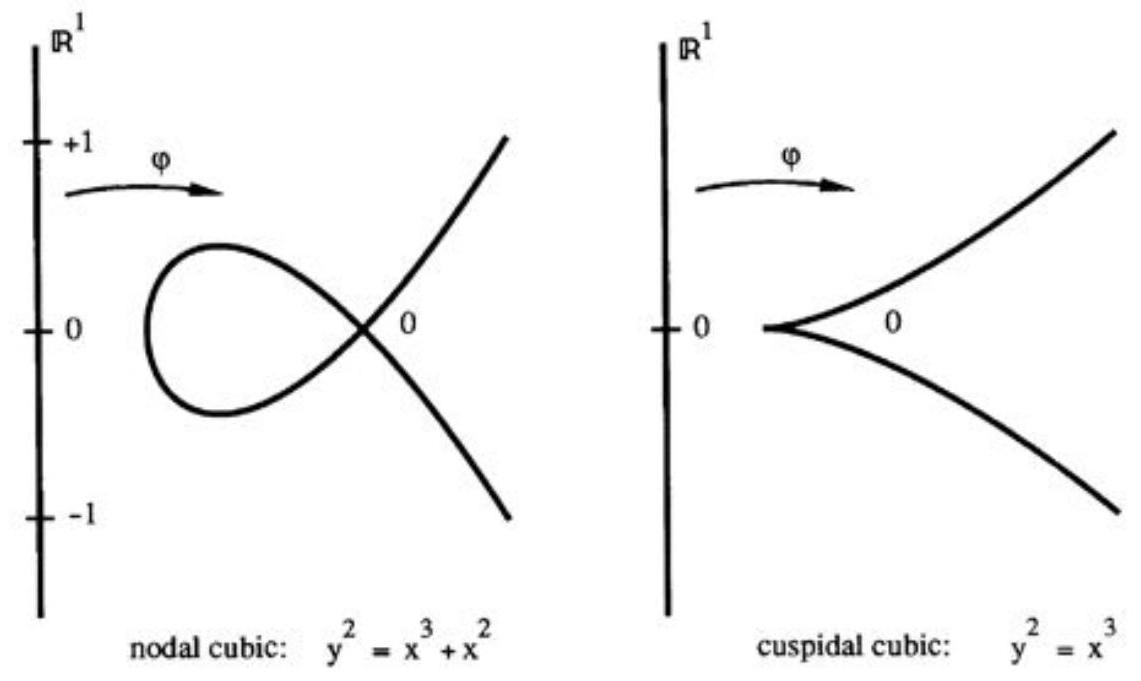
\includegraphics[max width=0.8\textwidth]{images/bo_d3lj80c601uc738kffi0_32_266_1160_1141_681_0.jpg}
\captionof{figure}{参数化三次曲线}
\end{center}
\hspace*{3em} 

请思考像、曲线以及映射 \(\varphi\) 的奇点.这些例子将在整个课程中反复出现，因此请花些时间研究这些方程；参见练习 2.1-2.

\section{曲线 \(y^2 = x(x-1)(x-\lambda)\) 没有有理参数化}

参数化曲线非常方便；例如，如果您对丢番图问题感兴趣，可能会期望有一个规则能给出所有的 \(\mathbb{Q}\)-值点，如 (1.1) 所示.(1.1) 的参数化形式为 \(x = f(t), y = g(t)\)，其中 \(f\) 和 \(g\) 是有理函数，即两个多项式的商.

\begin{theorem}
设 \(k\) 为特征不为 2 的域，且设 \(\lambda \in k\) 满足 \(\lambda \neq 0, 1\)；设 \(f, g \in k(t)\) 为满足以下条件的有理函数
\[
g^2 = f(f-1)(f-\lambda)
\]
则 \(f, g \in k\).
\end{theorem}

这等价于说，不存在任何由有理函数给出的非平凡映射 \(\mathbb{A}^1 \to C: y^2 = x(x-1)(x-\lambda)\).这反映了簇的一种非常强的“刚性”性质.

该定理的证明是在域 \(k(t)\) 上的算术，它利用了 \(k(t)\) 是唯一分解整环 (UFD) \(k[t]\) 的分式域这一事实.证明较长，您可以准备详细学习或暂时跳过（跳转至 2.4）.练习 2.12 中有一个通过在 \(\mathbb{Q}\) 上的算术进行不存在性证明的非常相似的例子.

\begin{proof}
利用 \(k[t]\) 是唯一分解整环的事实，我们写作
\[
f = p/q \quad \text{其中 } p, q \in k[t] \text{ 且互素，}
\]
\[
g = r/s \quad \text{其中 } r, s \in k[t] \text{ 且互素.}
\]
去分母后，原方程变为
\[
r^2 q^3 = s^2 p(p-q)(p-\lambda q)
\]
由于 \(r\) 和 \(s\) 互素，右侧的因子 \(s^2\) 必须整除 \(q^3\).同理，由于 \(p\) 和 \(q\) 互素，左侧的因子 \(q^3\) 必须整除 \(s^2\).因此，
\[
s^2 \mid q^3 \quad \text{且} \quad q^3 \mid s^2, \quad \text{从而 } s^2 = a q^3 \text{，其中 } a \in k^*
\]
（\(a\) 是 \(k[t]\) 的单位，因此属于 \(k\)）.
于是
\[
aq = (s/q)^2 \quad \text{是 } k[t] \text{ 中的一个平方.}
\]
此外，
\[
r^2 = a p(p-q)(p-\lambda q)
\]
因此通过考虑素因数分解，存在非零常数 \(b, c, d \in k\) 使得
\[
bp, \quad c(p-q), \quad d(p-\lambda q)
\]
都是 \(k[t]\) 中的平方.如果我能证明 \(p, q\) 是常数，那么根据前述内容，\(r, s\) 也将是常数，从而证明该定理.为了证明 \(p, q\) 是常数，设 \(K\) 为 \(k\) 的代数闭包；则 \(p, q \in K[t]\) 满足下一个引理的条件.
\end{proof}

\begin{lemma}
设 \(K\) 为代数闭域，\(p, q \in K[t]\) 为互素多项式.假设 4 个不同的线性组合（即对应于 4 个不同比值 \((\lambda : \mu) \in \mathbb{P}^1_K\) 的 \(\lambda p + \mu q\)）在 \(K[t]\) 中均为平方；则 \(p, q \in K\).
\end{lemma}

\begin{proof} (费马的“无限下降法”)
引理的假设和结论在用 \(p, q\) 替换为以下形式时不受影响
\[
p' = ap + bq, \quad q' = cp + dq,
\]
其中 \(a, b, c, d \in K\) 且 \(ad - bc \neq 0\).因此我们可以假设给定的 4 个平方是
\[
p, \quad p-q, \quad p-\lambda q, \quad q.
\]
则 \(p = u^2, q = v^2\)，且 \(u, v \in K[t]\) 互素.
现在通过反证法，假设 \(\max(\deg p, \deg q) > 0\) 且在所有满足引理条件的 \((p, q)\) 中取度数最小者.则
\[
p - q = u^2 - v^2 = (u-v)(u+v)
\]
和
\[
p - \lambda q = u^2 - \lambda v^2 = (u - \mu v)(u + \mu v)
\]
（其中 \(\mu = \sqrt{\lambda}\)）在 \(K[t]\) 中是平方.由 \(u, v\) 的互素性，我们得出 \(u-v, u+v, u-\mu v, u+\mu v\) 均为平方.这与 \(\max(\deg p, \deg q)\) 的最小性矛盾.
\end{proof}

\section{线性系统}\label{sec:linear-systems}

记 \(S_d = \{\text{次数为 } d \text{ 的齐次多项式}\} \subset k[X, Y, Z]\).任意元素 \(F \in S_d\) 可以唯一表示为
\[
F = \sum_{i+j+k=d} a_{ijk} X^i Y^j Z^k
\]
其中 \(a_{ijk} \in k\).这当然意味着 \(S_d\) 是一个以 \(k\) 为基的向量空间，其基为单项式：
\[
\begin{array}{cccc}
Z^d & & & \\
XZ^{d-1} & YZ^{d-1} & & \\
\vdots & & & \\
X^d & X^{d-1}Y & \dots & Y^d
\end{array}
\]
特别地，\(\dim S_d = \binom{d+2}{2}\).对于 \(P_1, \dots, P_n \in \mathbb{P}^2\)，定义
\[
S_d(P_1, \dots, P_n) = \{ F \in S_d \mid F(P_i) = 0 \text{ for } i=1, \dots, n \} \subset S_d.
\]
每个条件 \(F(P_i) = 0\)（更准确地说，是 \(F(X_i, Y_i, Z_i) = 0\)，其中 \(P_i = (X_i:Y_i:Z_i)\)）是对 \(F\) 的一个线性条件，因此 \(S_d(P_1, \dots, P_n)\) 是维数 \(\geq \binom{d+2}{2} - n\) 的向量空间.

\begin{lemma}
设 \(k\) 为无限域，且令 \(F \in S_d\).
\begin{enumerate}
    \item[(i)] 设 \(L \subset \mathbb{P}^2_k\) 为一条直线；若 \(F \equiv 0\) 在 \(L\) 上，则 \(F\) 在 \(k[X,Y,Z]\) 中可被 \(L\) 的方程整除.即，\(F = H \cdot F'\)，其中 \(H\) 是 \(L\) 的方程，且 \(F' \in S_{d-1}\).
    \item[(ii)] 设 \(C \subset \mathbb{P}^2_k\) 为非空非退化的圆锥曲线；若 \(F \equiv 0\) 在 \(C\) 上，则 \(F\) 在 \(k[X,Y,Z]\) 中可被 \(C\) 的方程整除.即，\(F = Q \cdot F'\)，其中 \(Q\) 是 \(C\) 的方程，且 \(F' \in S_{d-2}\).
\end{enumerate}
\end{lemma}

如果您认为这个命题显而易见，恭喜您的直觉：您刚刚猜到了零点定理 (Nullstellensatz) 的一个特例.现在请您自己寻找证明（或跳转至 2.6）.

\begin{proof}
(i) 通过坐标变换，我们可以假设 \(H = X\).那么对于任意 \(F \in S_d\)，存在唯一的表达式 \(F = X \cdot F'_{d-1} + G(Y, Z)\)：只需将所有含 \(X\) 的单项式归入第一个加数，剩下的必定是仅含 \(Y, Z\) 的多项式.现在
\[
F \equiv 0 \text{ on } L \iff G \equiv 0 \text{ on } L \iff G(Y, Z) = 0.
\]
最后一步成立是因为 (1.8)：若 \(G(Y, Z) \neq 0\)，则它在 \(\mathbb{P}^1_k\) 上最多有 \(d\) 个零点，而若 \(k\) 是无限的，则 \(\mathbb{P}^1_k\) 也是无限的.

(ii) 通过坐标变换，\(Q = XZ - Y^2\).现在我们来证明对于任意 \(F \in S_d\)，存在唯一的表达式
\[
F = Q \cdot F'_{d-2} + A(X, Z) + YB(X, Z)
\]
如果我们将 \(Y^2 = XZ - Q\) 代入 \(F\) 中所有出现的 \(Y^2\)，则关于 \(Y\) 的剩余项次数 \(\leq 1\)，因此其形式为 \(A(X, Z) + YB(X, Z)\).现在如同 (1.7)，\(C\) 是由 \(X=U^2, Y=UV, Z=V^2\) 给出的参数化圆锥曲线，因此
\[
F \equiv 0 \text{ on } C \iff A(U^2, V^2) + UVB(U^2, V^2) \equiv 0 \text{ on } C
\]
\[
\iff A(U^2, V^2) + UVB(U^2, V^2) = 0 \in k[U, V]
\]
\[
\iff A(X, Z) = 0 \text{ and } B(X, Z) = 0.
\]
这里最后的等价关系是通过分别考虑 \(A(U^2, V^2) + UVB(U^2, V^2)\) 中关于 \((U,V)\) 的偶次和奇次项得到的.
\end{proof}

练习 2.2 给出了类似的“显式”零点定理的例子.

\begin{corollary}
设 \(L: (H=0) \subset \mathbb{P}^2_k\) 为一条直线（或 \(C: (Q=0) \subset \mathbb{P}^2_k\) 为非退化圆锥曲线）；假设给定点 \(P_1, \dots, P_n \in \mathbb{P}^2_k\)，并考虑对某个固定的 \(d\)，\(S_d(P_1, \dots, P_n)\).则
\begin{enumerate}
    \item[(i)] 若 \(P_1, \dots, P_a \in L\)，\(P_{a+1}, \dots, P_n \notin L\) 且 \(a > d\)，则
    \[
    S_d(P_1, \dots, P_n) = H \cdot S_{d-1}(P_{a+1}, \dots, P_n).
    \]
    \item[(ii)] 如果 \(P_1, \dots, P_a \in C\)，\(P_{a+1}, \dots, P_n \notin C\) 且 \(a > 2d\)，则
    \[
    S_d(P_1, \dots, P_n) = Q \cdot S_{d-2}(P_{a+1}, \dots, P_n).
    \]
\end{enumerate}
\end{corollary}

\begin{proof}
(i) 如果 \(F\) 是 \(d\) 次齐次多项式，且曲线 \(D: (F=0)\) 在点 \(P_1, \dots, P_a\) 处与 \(L\) 相交，且满足 \(a > d\)，则根据 (1.9)，我们必须有 \(L \subset D\)，因此根据引理，\(F = H \cdot F'\)；现在由于 \(P_{a+1}, \dots, P_n \notin L\)，显然 \(F' \in S_{d-1}(P_{a+1}, \dots, P_n)\).(ii) 的证明完全相同.
\end{proof}

\begin{proposition}
设 \(k\) 是一个无限域，且有 \(P_1, \dots, P_8 \in \mathbb{P}^2_k\) 八个不同的点；假设 \(P_1, \dots, P_8\) 中没有 4 点共线，且没有 7 点位于同一条非退化二次曲线上，则
\[
\dim S_3(P_1, \dots, P_8) = 2.
\]
\end{proposition}

\begin{proof}
为简便起见，我们称一组点为“共二次曲线的”(conconic)，如果它们都位于同一条非退化二次曲线上.证明分为若干情况.

\textbf{主要情况：} 无 3 点共线，无 6 点共二次曲线.这是“一般位置”情况.

假设 \(\dim S_3(P_1, \dots, P_8) \geq 3\)，并令 \(P_9, P_{10}\) 是直线 \(L = P_1 P_2\) 上的不同点.则
\[
\dim S_3(P_1, \dots, P_{10}) \geq \dim S_3(P_1, \dots, P_8) - 2 \geq 1,
\]
因此存在 \(0 \neq F \in S_3(P_1, \dots, P_{10})\).根据推论 2.5，\(F = H \cdot Q\)，且满足 \(Q \in S_2(P_3, \dots, P_8)\).现在我们得到了与情况假设的矛盾：如果 \(Q\) 是非退化的，则 6 点 \(P_3, \dots, P_8\) 共二次曲线；而如果 \(Q\) 是一对直线或重直线，则至少 3 点共线.

\begin{center}
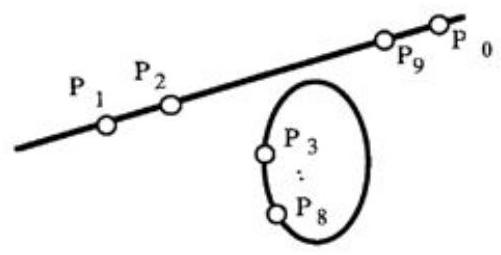
\includegraphics[max width=0.3\textwidth]{images/bo_d3lj80c601uc738kffi0_36_587_1142_501_255_0.jpg}
\captionof{figure}{一个可约三次曲线上的10个点}
\end{center}
\hspace*{3em} 

\textbf{第一退化情况：} 假设 \(P_1, P_2, P_3 \in L\) 共线，且令 \(L: (H=0)\).令 \(P_9\) 是直线 \(L\) 上的第 4 个点.则根据推论 2.5，
\[
S_3(P_1, \dots, P_9) = H \cdot S_2(P_4, \dots, P_8).
\]
此外，由于 \(P_4, \dots, P_8\) 中没有 4 点共线，根据推论 1.11，
\[
\dim S_2(P_4, \dots, P_8) = 1, \quad \text{那么} \quad \dim S_3(P_1, \dots, P_9) = 1,
\]
这意味着 \(\dim S_3(P_1, \dots, P_8) \leq 2\).

\textbf{第二退化情况：} 假设 \(P_1, \dots, P_6 \in C\) 共二次曲线，且 \(C: (Q=0)\) 是非退化二次曲线.然后选择与 \(P_1, \dots, P_6\) 不同的 \(P_9 \in Q\).再次根据推论 2.5，
\[
S_3(P_1, \dots, P_9) = Q \cdot S_1(P_7, P_8);
\]
直线 \(L = P_7 P_8\) 是唯一的，因此 \(S_3(P_1, \dots, P_9)\) 是由 \(QL\) 张成的一维空间，从而 \(\dim S_3(P_1, \dots, P_8) \leq 2\).
\end{proof}

\begin{corollary}[Cayley-Bacharach 定理]
设 \(C_1, C_2\) 为两条三次曲线，其交点由 9 个不同点组成，\(C_1 \cap C_2 = \{P_1, \dots, P_9\}\).则任何经过 \(P_1, \dots, P_8\) 的三次曲线 \(D\) 也必定经过 \(P_9\).
\end{corollary}

\begin{proof}
若 4 个点（例如 \(P_1, \dots, P_4\)）位于一条直线 \(L\) 上，则 \(C_1\) 和 \(C_2\) 各自与 \(L\) 相交于 \(\geq 4\) 个点，因此都包含 \(L\)，这与对 \(C_1 \cap C_2\) 的假设矛盾.出于完全相同的理由，不能有 7 个点共二次曲线.因此满足 (2.6) 的假设，故我们可以得出结论
\[
\dim S_3(P_1, \dots, P_8) = 2.
\]
这意味着两条三次曲线 \(C_1, C_2\) 的方程 \(F_1, F_2\) 构成 \(S_3(P_1, \dots, P_8)\) 的一组基.因此 \(D\) 的方程 \(G\) 可以写为 \(G = \lambda F_1 + \mu F_2\).现在 \(F_1, F_2\) 在 \(P_9\) 处为零，因此 \(G\) 在 \(P_9\) 处也为零.
\end{proof}

\section{平面三次曲线上的群运算}

设 \(k \subset \mathbb{C}\) 是 \(\mathbb{C}\) 的一个子域，\(F \in k[X,Y,Z]\) 是定义（非空）平面曲线 \(C: (F=0) \subset \mathbb{P}^2_k\) 的三次齐次多项式.假设 \(F\) 满足以下两个条件：
\begin{enumerate}
    \item[(a)] \(F\) 是不可约的（因此 \(C\) 不包含直线或二次曲线作为分量）；
    \item[(b)] 对每个点 \(P \in C\)，存在唯一一条直线 \(L \subset \mathbb{P}^2_k\)，使得 \(P\) 是 \(F|_L\) 的重根.
\end{enumerate}
注意，从几何角度看，条件 (b) 表示 \(C\) 应为非奇异的，所指的直线 \(L\) 是切线 \(L = T_P C\)（参见练习 2.3）.这将在第 6 章中成为非奇异性和簇的切空间一般定义的动机.

固定任意一点 \(O \in C\)，进行如下构造：

\textbf{构造}
\begin{enumerate}
    \item[(i)] 对 \(A \in C\)，令 \(\bar{A}\) 为 \(C\) 与直线 \(OA\) 的第三个交点；
    \item[(ii)] 对 \(A, B \in C\)，记 \(R\) 为 \(AB\) 与 \(C\) 的第三个交点，并通过 \(A+B = \bar{R}\) 定义和.
\end{enumerate}

\begin{center}
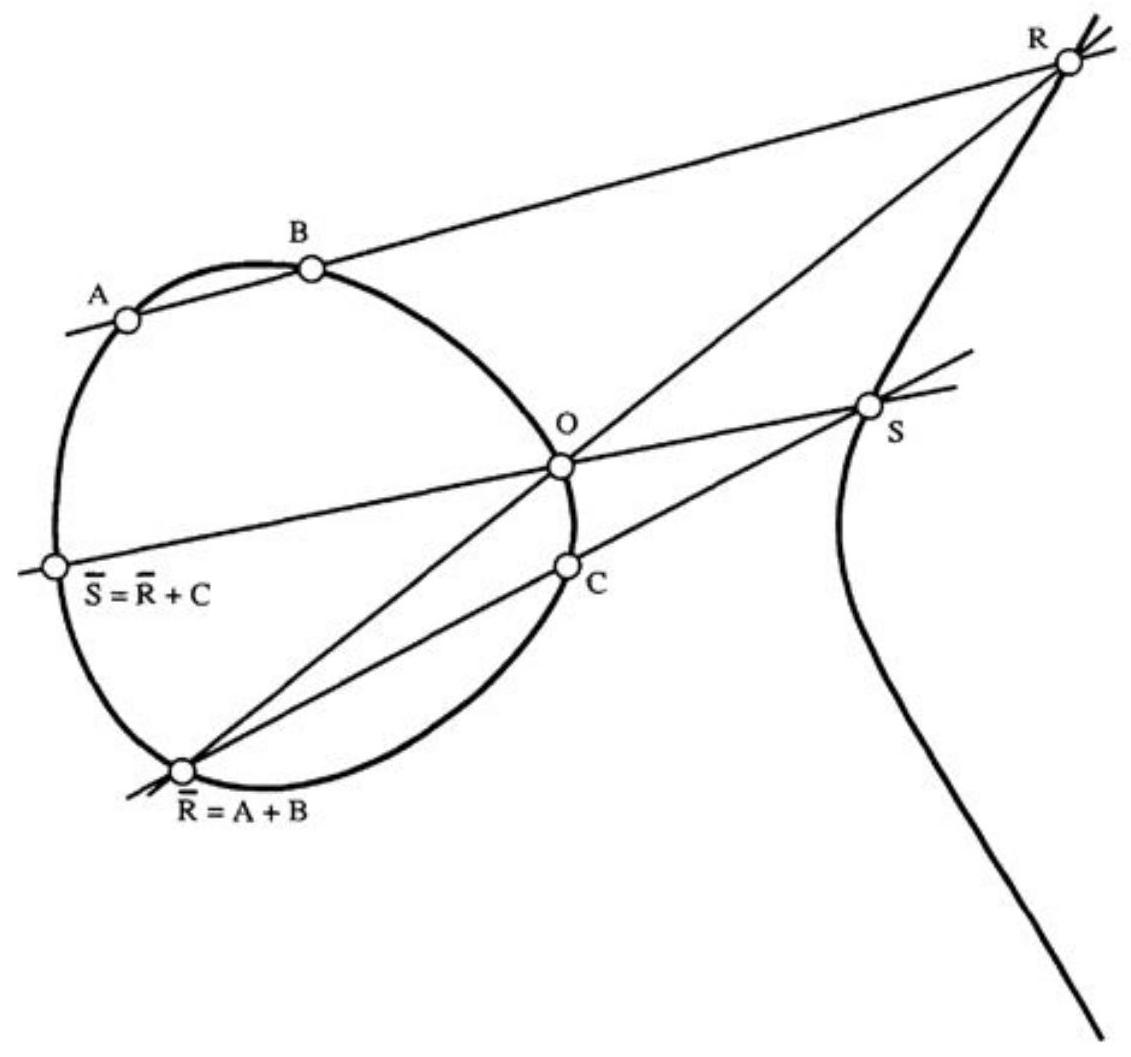
\includegraphics[max width=0.8\textwidth]{images/bo_d3lj80c601uc738kffi0_38_276_641_1131_1057_0.jpg}
\captionof{figure}{三次曲线及其群运算}
\end{center}
\hspace*{3em} 

\begin{theorem}
上述构造在 \(C\) 上定义了一个阿贝尔群运算，以 \(O\) 作为零元（单位元）.
\end{theorem}

\begin{proof}
结合律是关键；我们先从简单部分开始证明.

(I) \textbf{良定义性}：我们必须证明加法和逆元运算是良定义的.如果 \(P, Q \in C\) 是任意两点，那么要么 \(P \neq Q\)，此时直线 \(L = PQ \subset \mathbb{P}^2_k\) 是唯一确定的；要么 \(P = Q\)，此时根据假设 (b)，存在唯一一条直线 \(L \subset \mathbb{P}^2_k\) 使得 \(P\) 是 \(F|_L\) 的重根.无论哪种情况，\(F|_L\) 都是关于两个变量的三次齐次多项式，它有两个给定的 \(k\)-值零点.因此它可以分解为三个线性因子的乘积，故第三个剩余交点 \(R\) 是定义良好的，且其坐标属于 \(k\).注意，允许任意的 \(P=Q, P=R, Q=R\) 或 \(P=Q=R\)；这些在代数上对应于 \(F|_L\) 具有重根，在几何上对应于切点和拐点.

(II) \textbf{单位元}：验证给定点 \(O\) 是单位元完全是形式上的.由于 \(O, A, \bar{A}\) 共线，构造 \(O+A\) 包括取直线 \(L=OA\) 得到第三个交点 \(\bar{A}\)，然后用同一条直线 \(L=O\bar{A}\) 返回到 \(A\).

(III) \textbf{交换律}：\(A+B = B+A\) 留给读者作为练习.

(IV) \textbf{逆元}：首先定义构造中 (i) 所述的点 \(\bar{O}\)：设 \(L_0\) 为一条直线，使得 \(F|_{L_0}\) 在 \(O\) 处有重根，并定义 \(\bar{O}\) 为 \(L_0\) 与 \(C\) 的第三个交点.然后容易验证，对于每个 \(A \in C\)，\(A\) 的逆元是 \(\bar{O}A\) 与 \(C\) 的第三个交点.
\end{proof}

\section{一般情况下的结合律}

现在我们给出“足够一般”点的结合律证明.假设 \(A, B, C\) 是 \(C\) 上的三个给定点.则 \((A+B)+C = \bar{S}\) 的构造使用了 4 条直线（见上图）：
\[
L_1: ABR, \quad L_2: RO\bar{R}, \quad L_3: C\bar{R}S, \quad L_4: SO\bar{S}.
\]
而 \((B+C)+A = \bar{T}\) 的构造使用了 4 条直线：
\[
M_1: BCQ, \quad M_2: QO\bar{Q}, \quad M_3: A\bar{Q}T, \quad M_4: TO\bar{T}.
\]
我们想证明 \(\bar{S} = \bar{T}\)，为此只需证明 \(S=T\).考虑两个（可约的）三次曲线
\[
D_1 = L_1 \cup M_2 \cup L_3 \quad \text{和} \quad D_2 = M_1 \cup L_2 \cup M_3.
\]
根据构造，
\[
C \cap D_1 = \{A, B, C, O, R, \bar{R}, Q, \bar{Q}, S\},
\]
\[
C \cap D_2 = \{A, B, C, O, R, \bar{R}, Q, \bar{Q}, T\}.
\]
只要这 9 个点 \(A, B, C, O, R, \bar{R}, Q, \bar{Q}, S\) 均不相同，两条三次曲线 \(C\) 和 \(D_1\) 就满足推论 2.7 的条件.因此，\(D_2\) 必定经过 \(S\).如果 \(S\) 不在 \(D_2\) 的任何分量上，这唯一可能的情况是 \(S=T\).

要完成这个论证有多种方法.其中最彻底的方法是真正处理两条曲线的交点，考虑多重交点（大致用“交点理想”表示），与推论 2.7 对应的陈述是 Max Noether 引理（参见 [Fulton, pp. 120, 124]）.

\section{连续性证明}

我们简述一种“连续性”论证方法，它利用了 \(k \subset \mathbb{C}\) 的事实.记 \(C_\mathbb{C} \subset \mathbb{P}^2_\mathbb{C}\) 为复化曲线 \(C\)，即满足同一方程 \(F(X,Y,Z)=0\) 的复数比值集合 \((X:Y:Z)\).若结合律对所有 \(A, B, C \in C_\mathbb{C}\) 成立，则显然对 \(C\) 中的所有点也成立.因此，我们可以假设 \(k = \mathbb{C}\).

关心此事的读者不难找到以下两条陈述的证明（见练习 2.8）：

\begin{lemma}
\begin{enumerate}
    \item[(i)] \(A+B\) 是 \(A\) 和 \(B\) 的连续函数.
    \item[(ii)] 对于所有 \(A, B, C \in C\)，存在任意接近 \(A, B, C\) 的 \(A', B', C' \in C\)，使得由它们构造的 9 个点 \(A', B', C', O, R, \bar{R}, Q, \bar{Q}, S\) 均不相同.
\end{enumerate}
\end{lemma}

加法法则是映射 \(\varphi: C \times C \to C\)，由 \((A, B) \mapsto A+B\) 给出.根据 (i)，\(\varphi\) 是连续的，因此以下两个复合映射也是连续的：
\[
f = \varphi \circ (\varphi \times \operatorname{id}_C) \quad \text{和} \quad g = \varphi \circ (\operatorname{id}_C \times \varphi) : C \times C \times C \to C
\]
它们分别由 \((A, B, C) \mapsto (A+B)+C\) 和 \(A+(B+C)\) 给出.此外，根据 (ii)，使得构造中 9 个点均不同的三元组 \((A, B, C)\) 组成的子集 \(U \subset C \times C \times C\) 是稠密的.由上述论证，\(f\) 和 \(g\) 在 \(U\) 上重合，且因其连续性，故在任何地方都重合.

\textbf{备注}：连续性论证如其所述涉及 \(\mathbb{C}\) 的拓扑，因此并非纯代数的.事实上，加法映射 \(\varphi\) 是簇 (varieties) 的态射 \(\varphi: C \times C \to C\)，我们稍后将证明这一点（见 (4.14)）.其余论证也可以用这种纯代数形式重新表述：使得 9 个点互异的 \(C \times C \times C\) 的子集是 Zariski 拓扑下的稠密开集，而两个在稠密开集上重合的态射必定在全体上重合.（希望此备注能为课程其余部分提供有用的动机；若感到困惑，暂时可忽略.）

\section{帕斯卡定理 (神秘六边形)}

图中包含一个内接于二次曲线的六边形 \(ABCDEF \subset \mathbb{P}^2_k\)，其对边成对延长直至在点 \(P, Q, R\) 相交.假设图中的九点和六条直线均互不相同.

\begin{center}
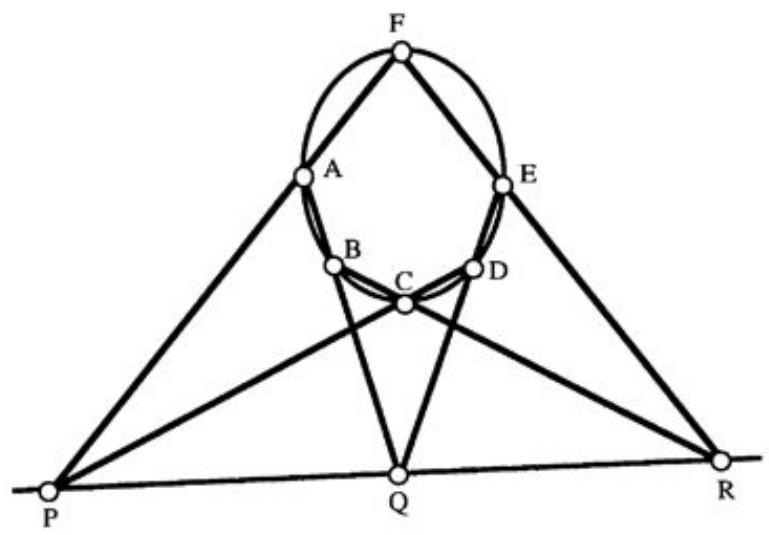
\includegraphics[max width=0.6\textwidth]{images/bo_d3lj80c601uc738kffi0_40_464_1080_769_535_0.jpg}
\captionof{figure}{神秘六边形}
\end{center}
\hspace*{3em} 

\begin{theorem}[帕斯卡定理]
六点 \(A, B, C, D, E, F\) 共二次曲线 \(\iff\) 三点 \(P, Q, R\) 共线.
\end{theorem}

这个著名定理是 (2.7) 的一个相当类似的应用，此处仅为趣味而给出.当然，也有其他证明方法，参见任何几何教材，例如 [Berger, 16.2.10 和 16.8.3-5].

\begin{proof}
在图中，考虑两组三条直线
\[
L_1: PAF, \quad L_2: QDE, \quad L_3: RBC,
\]
和
\[
M_1: PCD, \quad M_2: QAB, \quad M_3: REF.
\]
设 \(C_1 = L_1 \cup L_2 \cup L_3\) 和 \(C_2 = M_1 \cup M_2 \cup M_3\).显然 \(C_1\) 和 \(C_2\) 是两条三次曲线，且满足
\[
C_1 \cap C_2 = \{A, B, C, D, E, F, P, Q, R\}.
\]
\(\implies\): 假设 \(P, Q, R\) 共线，设 \(L\) 为过这三点的直线.设 \(\Gamma\) 为经过 \(A, B, C, D, E\) 的二次曲线（其存在性和唯一性由命题 1.11 保证）.则 \(L \cup \Gamma\) 是一个经过 8 个点 \(A, B, C, D, E, P, Q, R\) 的三次曲线.依据 (2.7)，它必包含第 9 个点 \(F\).根据假设，\(F \notin L\)，因此必然有 \(F \in \Gamma\)，证明这六点共二次曲线.

\(\impliedby\): 反之，假设 \(A, B, C, D, E, F\) 位于二次曲线 \(\Gamma\) 上.设 \(L = PQ\).则 \(L \cup \Gamma\) 是经过 \(A, B, C, D, E, F, P, Q\) 这 8 个点的三次曲线，故根据 (2.7) 它必经过第 9 个点 \(R\).现在 \(R\) 不可能位于二次曲线 \(\Gamma\) 上（否则 \(\Gamma\) 是两条直线的组合，且图中的六条直线中必有重合），因此 \(R \in L\)，即 \(P, Q, R\) 共线.
\end{proof}

\section{拐点与标准形}

\(\mathbb{P}^2_\mathbb{R}\) 或 \(\mathbb{P}^2_\mathbb{C}\) 中的任意非奇异三次曲线均可经过射影变换化为标准形（魏尔斯特拉斯范式）
\[
Y^2 Z = X^3 + aXZ^2 + bZ^3,
\]
或其仿射形式
\[
y^2 = x^3 + ax + b.
\]
现在考虑上述曲线 \(C\).它与无穷远直线 \(L: (Z=0)\) 相交于何处？只需将 \(Z=0\) 代入定义多项式 \(F = -Y^2 Z + X^3 + aXZ^2 + bZ^3\)，得到 \(F|_L = X^3\).这意味着 \(F|_L\) 在点 \(O = (0:1:0)\) 处有三重根.为理解其几何意义，设 \(Y=1\)，得到以 \((0:1:0)\) 为中心的仿射坐标 \((x, z)\) 下的方程：
\[
z = x^3 + axz^2 + bz^3.
\]
该曲线在原点附近可被 \(z = x^3\) 高度精确地近似.

\begin{center}
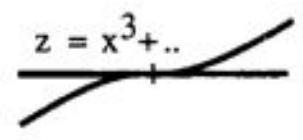
\includegraphics[max width=0.2\textwidth]{images/bo_d3lj80c601uc738kffi0_41_793_1592_303_140_0.jpg}
\captionof{figure}{拐点}
\end{center}
\hspace*{3em} 

这表示 \(C\) 在 \((0:1:0)\) 处有一个拐点.更一般地，曲线 \(C\) 上的拐点 \(P\) 定义为存在一条直线 \(L \subset \mathbb{P}^2_k\)，使得 \(F|_L\) 在 \(P\) 处有重数 \(\geq 3\) 的根（参见练习 2.9；实际上根据 (2.8, b) 必然有 \(L = T_P C\)，重数由 (1.9) 确定）.用定义方程的导数和二阶导数来解释这一点并不难：例如，如果定义方程是 \(y = f(x)\)，那么拐点的条件就是 \(\frac{d^2 f}{dx^2}(P) = 0\).这在图中对应曲线从“下凹”到“上凹”的转变.关于平面曲线存在拐点的一般判据可用 Hessian 矩阵表示，详见 [Fulton, p. 116] 或练习 7.3 (iii).

可以证明（参见练习 2.10），反之若平面三次曲线 \(C\) 有一个拐点，则其方程可化为上述的标准形式.

\section{简化的群运算律}

标准形式对于群运算律极为方便：取拐点 \(O = (0:1:0)\) 作为单位元.在此条件下，群运算律特别简洁，原因如下：
\begin{enumerate}
    \item[(a)] \(C = \{O\} \cup C_0\)，其中 \(C_0\) 是仿射曲线 \(y^2 = x^3 + ax + b\).因此将 \(C\) 视为仿射曲线是合理的，偶尔提及无穷远点 \(O\)，即群运算的零元.
    \item[(b)] 通过 \(O\) 的直线是构造群运算 (2.8, i) 的主要元素.这些直线在射影意义下由 \(X = \lambda Z\) 给出，在仿射意义下由 \(x = \lambda\) 给出.任意此类直线与 \(C\) 相交于点 \((\lambda, \pm \sqrt{\lambda^3 + a\lambda + b})\) 及无穷远点 \(O\).因此若 \(P = (x, y)\)，则 (2.8, i) 中构造的点 \(\bar{P}\) 为 \((x, -y)\).故 \(P \mapsto \bar{P}\) 是曲线 \(C_0\) 关于 \(x\)-轴的自然对称 \((x, y) \mapsto (x, -y)\).
\end{enumerate}

\begin{center}
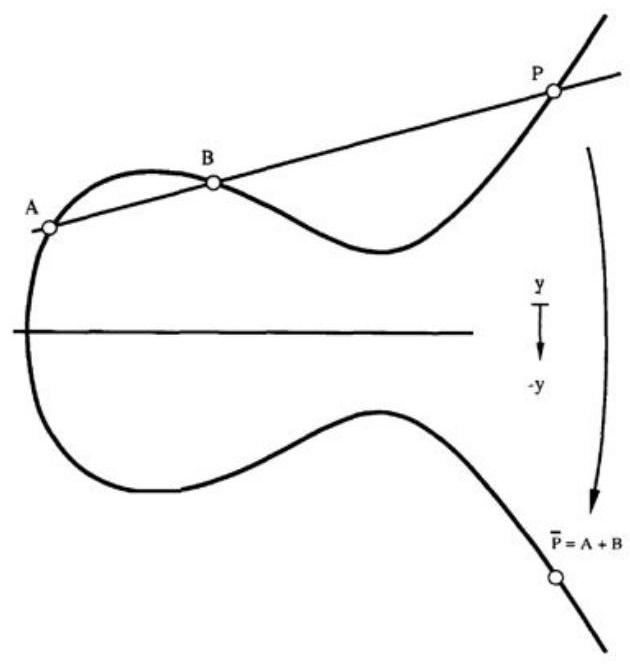
\includegraphics[max width=0.4\textwidth]{images/bo_d3lj80c601uc738kffi0_42_528_1157_630_664_0.jpg}
\captionof{figure}{以 \(x\) 轴为反射轴的取负运算}
\end{center}
\hspace*{3em} 

\begin{enumerate}
    \item[(c)] 群运算 (2.8, IV) 的逆元通过 \(\bar{O}\) 描述，该点是 \(C\) 与其在 \(O\) 处的切线的第三个交点.在本例中，该切线是无穷远直线 \(L: (Z=0)\)，且 \(L \cap C = 3O\)，因此 \(\bar{O} = O\).群运算的逆元简化为 \(-P = \bar{P}\).
\end{enumerate}

我们现在可以将群运算律重新表述为定理 2.8 的一个大大简化的版本：

\begin{theorem}
设 \(C\) 是标准形式的三次曲线；则在 \(C\) 上存在唯一的群运算，使得 \(O = (0:1:0)\) 是单位元，逆元由 \((x, y) \mapsto (x, -y)\) 给出，且对所有 \(P, Q, R \in C\)，
\[
P + Q + R = O \iff P, Q, R \text{ 共线.}
\]
\end{theorem}

\section{第二章习题}

\begin{exercise}
设 \(C: y^2 = x^3 + x^2 \subset \mathbb{R}^2\).证明通过原点 \((0,0)\) 的一条变量直线与 \(C\) 还有一个交点，由此推导出 (2.1) 中给出的 \(C\) 的参数化.对 \(y^2 = x^3\) 和 \(x^3 = y^3 - y^4\) 也做同样的操作.
\end{exercise}

\begin{exercise}
设 \(\varphi: \mathbb{R}^1 \to \mathbb{R}^2\) 是由 \(t \mapsto (t^2, t^3)\) 给出的映射.直接证明任何在像 \(C = \varphi(\mathbb{R}^1)\) 上为零的多项式 \(f \in \mathbb{R}[X, Y]\) 都能被 \(Y^2 - X^3\) 整除.[提示：使用引理 2.5 中的方法.] 确定域 \(k\) 需具备何种性质才能保证对由相同公式给出的 \(\varphi: k \to k^2\) 结果成立.
对 \(t \mapsto (t^2 - 1, t^3 - t)\) 也做同样的操作.
\end{exercise}

\begin{exercise}
设 \(C: (f=0) \subset k^2\)，且设 \(P=(a,b) \in C\).假设 \(\frac{\partial f}{\partial x}(P) \neq 0\) 或 \(\frac{\partial f}{\partial y}(P) \neq 0\).证明直线
\[
L: \frac{\partial f}{\partial x}(P) \cdot (x-a) + \frac{\partial f}{\partial y}(P) \cdot (y-b) = 0
\]
是 \(C\) 在 \(P\) 处的切线，即 \(k^2\) 中唯一一条使得 \(f|_L\) 在 \(P\) 处有重根的直线（详见 (6.1) 中的推导）.
\end{exercise}

\begin{exercise}
设 \(C: y^2 = x^3 + 4x\)，采用简化的群运算 (2.13).证明 \(C\) 在 \(P=(2,4)\) 处的切线经过原点 \((0,0)\)，由此推断 \(P\) 是该群运算中的一个 4 阶点.
\end{exercise}

\begin{exercise}
设 \(C: y^2 = x^3 + ax + b \subset \mathbb{R}^2\) 是非奇异的.找出群运算中所有的 2 阶点，并理解它们构成的群（需考虑两种情况）.然后几何上说明如何寻找 \(C\) 上所有的 4 阶点.
\end{exercise}

\begin{exercise}
设 \(C: y^2 = x^3 + ax + b \subset \mathbb{R}^2\).编写一个计算机程序绘制 \(C\) 的部分图形，并计算群运算.程序应提示输入两点 \(A\) 和 \(B\) 的坐标，随后绘制直线并输出 \(A+B\) 的坐标.（使用实数变量.）
\end{exercise}

\begin{exercise}
设 \(C: y^2 = x^3 + ax + b \subset k^2\).若 \(A=(x_1, y_1)\) 且 \(B=(x_2, y_2)\)，说明如何将 \(A+B\) 的坐标表示为 \(x_1, y_1, x_2, y_2\) 的有理函数.[提示：若 \(F(X)\) 是三次多项式且已知两个根，则可通过观察 \(F\) 的一个系数找到第三个根.此题答案不唯一，因为有多种正确的有理函数表达式.一个解见 (4.14).]
\end{exercise}

\begin{exercise}
通过写出 \(C\) 在 \(A\) 处切线的方程，求出群运算中 \(C\) 上 \(2A\) 的公式，并验证当 \(B\) 趋近于 \(A\) 时，该公式是 \(A+B\) 公式的极限.[提示：使用练习 2.7，必要时参考 (4.14).]
\end{exercise}

\begin{exercise}
设 \(x, z\) 为 \(k^2\) 上的坐标，且设 \(f \in k[x, z]\).将 \(f\) 写成
\[
f = a + bx + cz + dx^2 + exz + fz^2 + \dots
\]
用系数 \(a, b, c, \dots\) 表示必须满足的条件，以保证
\begin{enumerate}
    \item[(i)] \(P=(0,0) \in C: (f=0)\);
    \item[(ii)] \(C\) 在 \(P\) 处的切线是 \(z=0\);
    \item[(iii)] \(P\) 是 \(C\) 的一个拐点，且切线为 \(z=0\).
\end{enumerate}
(回顾 (2.12)，若切线 \(L\) 存在，且 \(f|_L\) 在 \(P\) 处至少有三重根，则 \(P \in C\) 为拐点.)
\end{exercise}

\begin{exercise}
设 \(C \subset \mathbb{P}^2_k\) 为平面三次曲线，假设 \(P \in C\) 是一个拐点.证明通过在 \(\mathbb{P}^2_k\) 中变换坐标，可以将 \(C\) 化为标准形式
\[
Y^2 Z = X^3 + aX^2 Z + bXZ^2 + cZ^3.
\]
[提示：取坐标使得 \(P=(0:1:0)\) 及拐点切线为 \(Z=0\).利用前一题，在局部坐标 \((x,z)\) 中，\(Y\) 将以二次项 \(Y^2 Z\) 出现，其余仅线性出现.然后通过配方法消去 \(Y\) 中的线性项.]
\end{exercise}

\begin{exercise}[尖点三次曲线上的群运算]
考虑曲线 \(C: z = x^3 \subset k^2\).\(C\) 是双射映射 \(\varphi: k \to C\)（由 \(t \mapsto (t, t^3)\) 给出）的像，因此继承了加法群 \(k\) 的群结构.证明这是 \(C\) 上唯一的群运算，使得 \((0,0)\) 为单位元且
\[
P+Q+R=0 \iff P, Q, R \text{ 共线}
\]
对于 \(P, Q, R \in C\).[提示：你可能会发现恒等式
\[
\det \begin{vmatrix} 1 & a & a^3 \\ 1 & b & b^3 \\ 1 & c & c^3 \end{vmatrix} = (a-b)(b-c)(c-a)(a+b+c).
\]
在射影几何的术语中，\(C\) 是曲线 \(Y^2 Z = X^3\)，即我们熟悉的在原点有尖点且在 \((0:1:0)\) 有拐点的曲线.本题的关键是，通常的构造在奇点的补集上给出了群运算.]
\end{exercise}

\begin{exercise}[由莱昂纳多·斐波那契于公元1220年提出]
证明对于 \(u, v \in \mathbb{Z}\)，
\[
u^2+v^2 \text{ 和 } u^2-v^2 \text{ 均为平方数 } \implies v=0.
\]
提示 (由皮埃尔·德·费马提供，见 J.W.S. Cassels, J. London Math. Soc. 41 (1966), p. 207):
\begin{enumerate}
    \item[第一步] 化简为求解 \(x^2 = u^2+v^2, y^2 = u^2-v^2\)，其中 \(x, y, u, v \in \mathbb{Z}\) 两两互质.
    \item[第二步] 模 4 的考虑表明 \(x, y, u\) 是奇数，\(v\) 是偶数.
    \item[第三步] 因式分解方程 \((x-u)(x+u)=v^2\) 和 \((u-y)(u+y)=v^2\).
    \item[第四步] 证明 \(x-u=2v_1^2, u-y=2u_1^2, x-y=2x_1^2\) 和 \(2u-x-y=2y_1^2\)，其中 \(u_1, v_1, x_1, y_1 \in \mathbb{Z}\).
    \item[第五步] 证明 \(u_1, v_1, x_1, y_1\) 是原方程的另一个解，且满足 \(v_1 < v\)，并通过“无限下降法”推导出矛盾.
\end{enumerate}
请将此论证与 (2.2) 的证明进行比较，后者更简单，仅因为我们不必处理 2 的幂次问题.
\end{exercise}